% Regenerate from this directory:
% latex -interaction=nonstopmode -halt-on-error incexcp.tex
% dvisvgm --no-fonts --exact --bbox=papersize --output=incexcp.svg incexcp.dvi
\documentclass[tikz,border=4pt]{standalone}
\definecolor{setA}{RGB}{180,0,0}
\definecolor{setB}{RGB}{0,0,210}
\definecolor{setC}{RGB}{0,130,0}
\newcommand{\setA}{\textcolor{setA}{A}}
\newcommand{\setB}{\textcolor{setB}{B}}
\newcommand{\setC}{\textcolor{setC}{C}}
\begin{document}
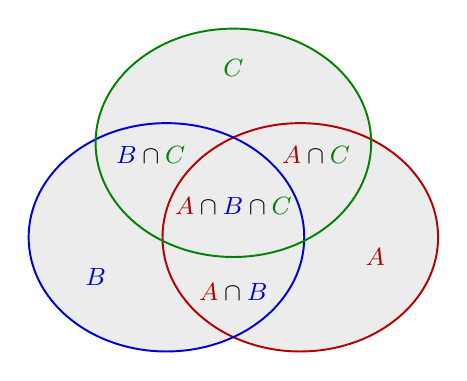
\begin{tikzpicture}[line width=0.7pt,font=\small]
  \coordinate (A) at (3.7,1.65);
  \coordinate (B) at (2,1.65);
  \coordinate (C) at (2.85,2.85);
  % Fill the union before drawing boundaries so every overlap remains visible.
  \foreach \centre in {A,B,C}
    \fill[gray!15] (\centre) ellipse[x radius=1.75cm,y radius=1.45cm];
  \draw[setA] (A) ellipse[x radius=1.75cm,y radius=1.45cm];
  \draw[setB] (B) ellipse[x radius=1.75cm,y radius=1.45cm];
  \draw[setC] (C) ellipse[x radius=1.75cm,y radius=1.45cm];
  % Labels occupy the seven nonempty Venn regions, as in the original diagram.
  \node at (4.65,1.4) {$\setA$};
  \node at (1.1,1.15) {$\setB$};
  \node at (2.85,3.8) {$\setC$};
  \node at (2.85,0.95) {$\setA\cap\setB$};
  \node at (3.9,2.7) {$\setA\cap\setC$};
  \node at (1.8,2.7) {$\setB\cap\setC$};
  \node at (2.85,2.05) {$\setA\cap\setB\cap\setC$};
\end{tikzpicture}
\end{document}
